\documentclass{article}
\usepackage{harvard}
\usepackage{hyperref}
\usepackage{graphics}
\usepackage{amsmath}
\usepackage{indentfirst}
\usepackage[utf8]{inputenc}
\usepackage[top=1in, bottom=1in, left=1in, right=1in]{geometry}
\DeclareMathOperator{\var}{var}
% \VignetteIndexEntry{Using GrpSeqBnds}
\usepackage{/usr/local/lib64/R/share/texmf/Sweave}
\begin{document}


\title{Calculation of Efficacy and Futiltiy Boundaries using GrpSeqBnds (Version 1.15)}
\author{Grant Izmirlian}
\maketitle

\section{Introduction}
The function $\mathbf{GrpSeqBnds}$ computes efficacy and futility boundaries given the
stipulation of the information fraction, total type I and type II error probabilities and method
of boundary construction.  The efficacy and futility boundaries can be constructed either
simulataneously or one at a time.  The function also allows for two information scales.



The following sequence of variance fractions resulted from a trial with 7 or so years of accrual
and maximum follow-up of 20 years using the stopped Fleming-Harrington weights, $\mathbf{SFH}(0,1,10)$.
\begin{Schunk}
\begin{Sinput}
> frac <- c(0.006995655, 0.01444565, 0.02682463, 0.04641363, 
+     0.0585665, 0.07614902, 0.1135391, 0.168252, 0.2336901, 
+     0.3186155, 0.4164776, 0.5352199, 0.670739, 0.8246061, 
+     1)
\end{Sinput}
\end{Schunk}

The same settings resulted in the following sequence of event ratios:

\begin{Schunk}
\begin{Sinput}
> frac.ii <- c(0.1494354, 0.1972965, 0.2625075, 0.3274323, 
+     0.3519184, 0.40231, 0.4673037, 0.5579035, 0.6080742, 
+     0.6982293, 0.7671917, 0.8195019, 0.9045182, 0.9515884, 
+     1)
\end{Sinput}
\end{Schunk}

The $\mathbf{SFH}(0,1,10)$ statistic together with an average effect of $20\%$
reduction in risk, subjected to contamination and dropout, resulted in the
following sequence of drift function values.  Recall that the drift function
is the expected value of the statistic at a given alternative hypothesis.  The
scale is always the same as the main (first) information scale.  

\begin{Schunk}
\begin{Sinput}
> drift <- c(0.06214444, 0.1061856, 0.1731267, 0.2641265, 
+     0.3105231, 0.3836636, 0.5117394, 0.6918584, 0.8657705, 
+     1.091984, 1.311094, 1.538582, 1.818346, 2.081775, 
+     2.345386)
\end{Sinput}
\end{Schunk}

\begin{itemize}
  \item[1.]{{\bf One Sided Efficacy Boundary}\\
    In this example, we calculate a one sided efficacy boundary at each of 15 analyses which
    will occur at the given (known) variance ratios, and we use the variance ratio for type I
    error probability spending, with a total type I error probabilty of 0.05, using the
    Lan-Demets method with Obrien-Fleming spending (the default). We plot the resulting boundary.
    
\begin{Schunk}
\begin{Sinput}
> example.1 <- GrpSeqBnds(frac = frac, EfficacyBoundary = LanDemets(alpha = 0.05, 
+     spending = ObrienFleming))
\end{Sinput}
\end{Schunk}

\begin{Schunk}
\begin{Sinput}
> plot(example.1)
\end{Sinput}
\end{Schunk}
  }

  \begin{figure}
  \begin{center}
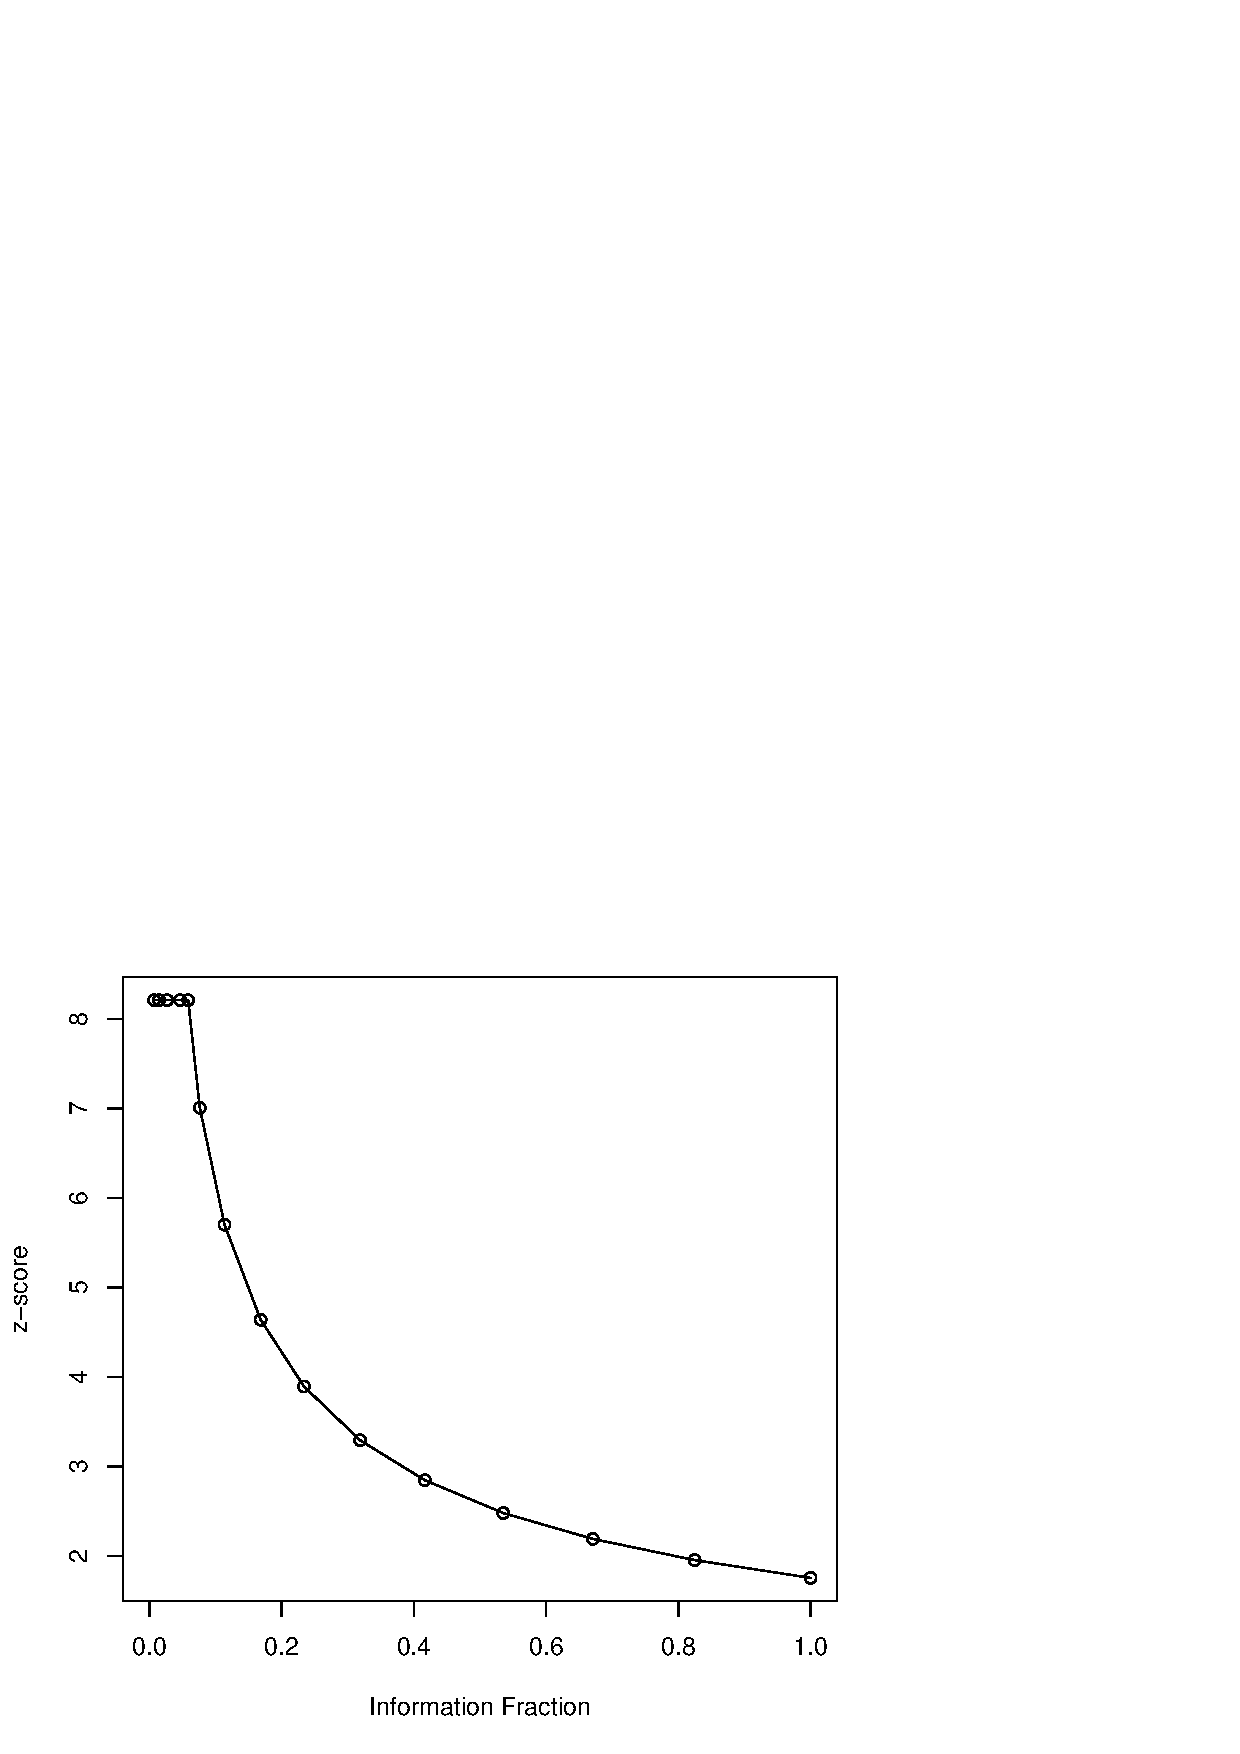
\includegraphics{GrpSeqBnds-vignette-1-incl-ex1-plot}
  \end{center}
  \caption{One-sided efficacy boundary constructed via the Lan-Demets method,
    using the O'Brien-Fleming error probability spending function, with total
    type I error probability set to $0.05$}
  \label{fig:ex1}
  \end{figure}

  \item[2.]{{\bf One Sided Efficacy and Futility Boundaries}\\
    In this call, we calculate a one sided efficacy boundary at each of 15 analyses which will
    occur at the given (known) variance ratios, and we use the variance ratio for type I and
    type II error probability spending, with a total type I error probabilty of 0.05 and a total
    type II error probability of 0.10, using the Lan-Demets method with Obrien-Fleming spending
    (the default) for both efficacy and futilty. We plot the resulting boundaries, and verify
    their accuracy via the $\mathbf{SimGSB}$ function.

\begin{Schunk}
\begin{Sinput}
> example.2 <- GrpSeqBnds(frac = frac, EfficacyBoundary = LanDemets(alpha = 0.05, 
+     spending = ObrienFleming), FutilityBoundary = LanDemets(alpha = 0.1, 
+     spending = ObrienFleming), drift = drift)
> SimGSB(example.2)
\end{Sinput}
\begin{Soutput}
          eI.est       eI.act eII.est      eII.act
0.006996 0.00000 1.000000e-15 0.00000 1.000000e-15
0.01445  0.00000 2.000000e-15 0.00000 2.000000e-15
0.02682  0.00000 3.000000e-15 0.00000 3.000000e-15
0.04641  0.00000 4.000000e-15 0.00000 2.559608e-14
0.05857  0.00000 5.000000e-15 0.00000 1.070201e-11
0.07615  0.00000 1.229520e-12 0.00000 2.512057e-09
0.1135   0.00000 6.002701e-09 0.00000 1.052745e-06
0.1683   0.00000 1.768361e-06 0.00003 6.071218e-05
0.2337   0.00001 5.026046e-05 0.00054 6.675519e-04
0.3186   0.00051 5.160593e-04 0.00332 3.567972e-03
0.4165   0.00240 2.389040e-03 0.01043 1.081021e-02
0.5352   0.00777 7.382981e-03 0.02436 2.455480e-02
0.6707   0.01752 1.670406e-02 0.04443 4.460067e-02
0.8246   0.03207 3.089949e-02 0.06905 7.008565e-02
1        0.05163 5.000000e-02 0.22989 2.306475e-01
\end{Soutput}
\end{Schunk}

\begin{Schunk}
\begin{Sinput}
> plot(example.2)
\end{Sinput}
\end{Schunk}
  }

  \begin{figure}
  \begin{center}
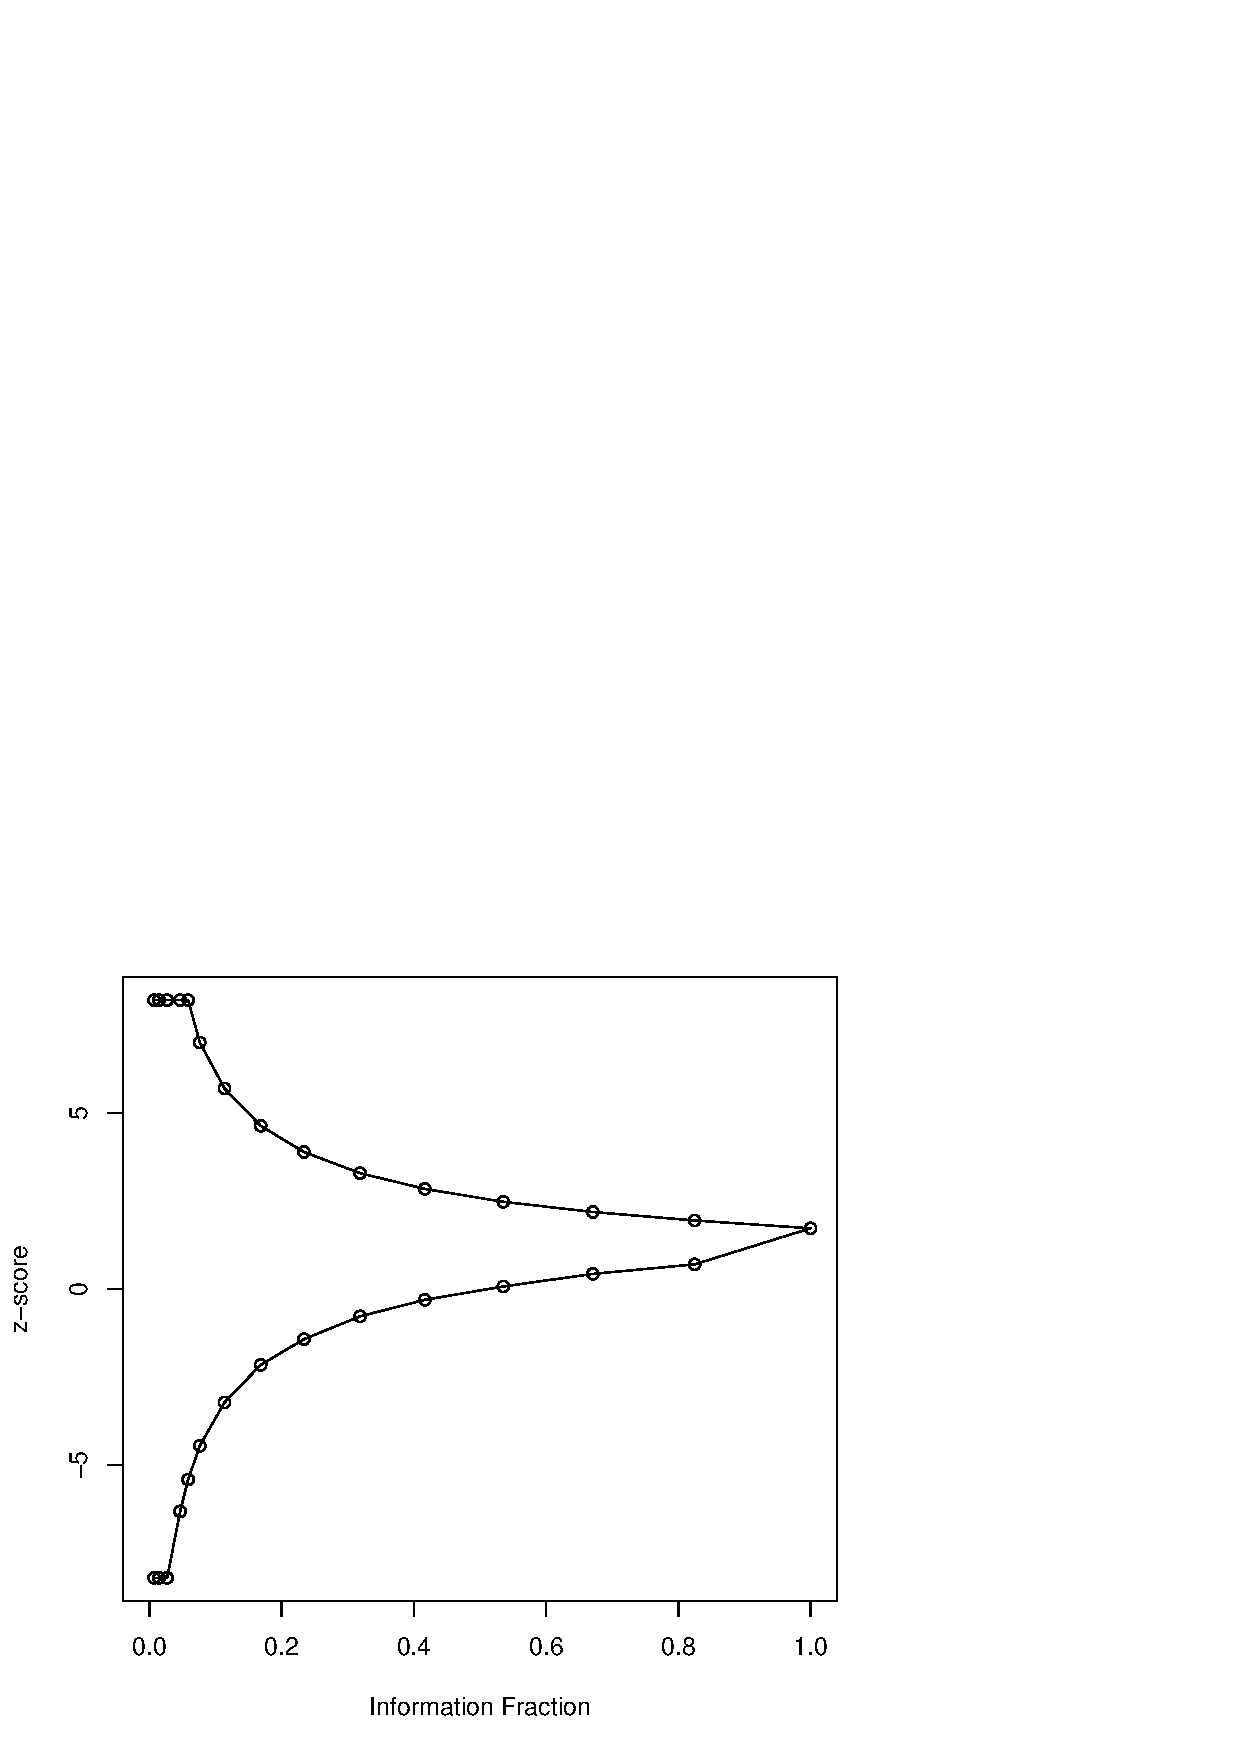
\includegraphics{GrpSeqBnds-vignette-1-incl-ex2-plot}
  \end{center}
  \caption{One-sided efficacy and futility boundaries constructed via the Lan-Demets method,
    using the O'Brien-Fleming error probability spending function, with total type I and type II
    error probabilities set to $0.05$ and $0.10$, respectively. The futility boundary is
    constructed relative to the  alternative hypothesis corresponding to the drift sequence above.}
  \label{fig:ex2}
  \end{figure}

\item[3.]{{\bf One Sided Efficacy and Futility Boundaries with Two information Scales}\\
    The following example illustrates the use of the two information scales. Note that
    according to the theory, the concept ``information fraction'' refers to the ratio of
    variances of the current statistic to the statistic at the end of the trial.  In many
    circumstances, the variance of the test statistic at the end of the trial is known based
    upon the original design. For example, if the test statistic is the ordinary (unweighted)
    log-rank statistic, the arms are balanced, and censoring and event rates are relatively
    rare, then the variance at the end of the trial is roughly one quarter of the total
    expected events so that the variance ratio equals the ratio of current observed events to
    the total expected.  However, with the introduction of a weighting function, the timing of
    the events can drastically alter the value of the end of trial variance.
    
    This phenomenon led Lan and Demets to introduce the use of two information scales.  In order
    to understand the nature of this innovation, consider that the information fraction serves
    two distinct purposes: (i) in the spending of errror probability and (ii) in the
    transformation of the sequence of observed test statistics to a process having normally
    distributed independent increments with variance linear in information (Brownian paths). The
    key behind their innovation was the observation that one could use separate information
    scales for each one of these purposes. First, instead of normalizing the sequence of current
    and previously recorded statistics to have unit variance at the end of the trial, which
    required knowledge of the end of trial variance, one could normalize to have unit variance
    at the current analysis. This still results in Brownian paths.  However, the information
    scale on which error probability is spent must be monotone increasing from 0 to 1 throughout
    the duration of the trial, but there is no real reason to require this scale of information
    to grow as the variance ratio.  In fact, one may stipulate any scale.  The original reason
    that the two scales were specified on the single variance scale was so that the resulting
    procedure was equivalent to continuous monitoring of the test statistic (by the reflection
    principle).  
    
    In the following example, suppose that we are performing the 7th interim analysis. We don't
    know what the variance will be at the end of the trial, so we normalize variances of the
    current and previous statistics by the variance of the current statistic.  This is
    equivalent to the following length 7 vector of variance ratios:
    
\begin{Schunk}
\begin{Sinput}
> frac7 <- frac[1:7]/frac[7]
\end{Sinput}
\end{Schunk}
    To proceed under the "unknown variance at end of trial" case, we must use a second
    scale for spending type I and II error probabilty. Unlike the above scale
    which is renormalized at each analysis to have value 1 at the current analysis, the
    alpha spending scale must be monotone increasing and attain the value 1 only at the
    end of the trial. A natural choice is the event ratio, which is known in advance if
    the trial is run until a required number of events is obtained, a so called
    maximum information trial:

\begin{Schunk}
\begin{Sinput}
> frac7.ii <- frac.ii[1:7]
\end{Sinput}
\end{Schunk}

    the first seven values of the drift function

\begin{Schunk}
\begin{Sinput}
> drift7 <- drift[1:7]/frac[7]^0.5
\end{Sinput}
\end{Schunk}

\begin{Schunk}
\begin{Sinput}
> example.3 <- GrpSeqBnds(frac = frac7, frac.ii = frac7.ii, 
+     EfficacyBoundary = LanDemets(alpha = 0.05, spending = ObrienFleming), 
+     FutilityBoundary = LanDemets(alpha = 0.1, spending = ObrienFleming), 
+     drift = drift7)
> SimGSB(example.3)
\end{Sinput}
\begin{Soutput}
        eI.est       eI.act eII.est      eII.act
0.1494 0.00000 3.974892e-07 0.00001 2.090403e-05
0.1973 0.00002 1.021661e-05 0.00015 2.129657e-04
0.2625 0.00010 1.305582e-04 0.00131 1.325597e-03
0.3274 0.00061 6.143221e-04 0.00406 4.046323e-03
0.3519 0.00084 9.534929e-04 0.00547 5.558965e-03
0.4023 0.00175 2.001124e-03 0.00952 9.506958e-03
0.4673 0.00388 4.142034e-03 0.01663 1.612043e-02
\end{Soutput}
\end{Schunk}

\begin{Schunk}
\begin{Sinput}
> plot(example.3)
\end{Sinput}
\end{Schunk}
  }
  
  \begin{figure}
  \begin{center}
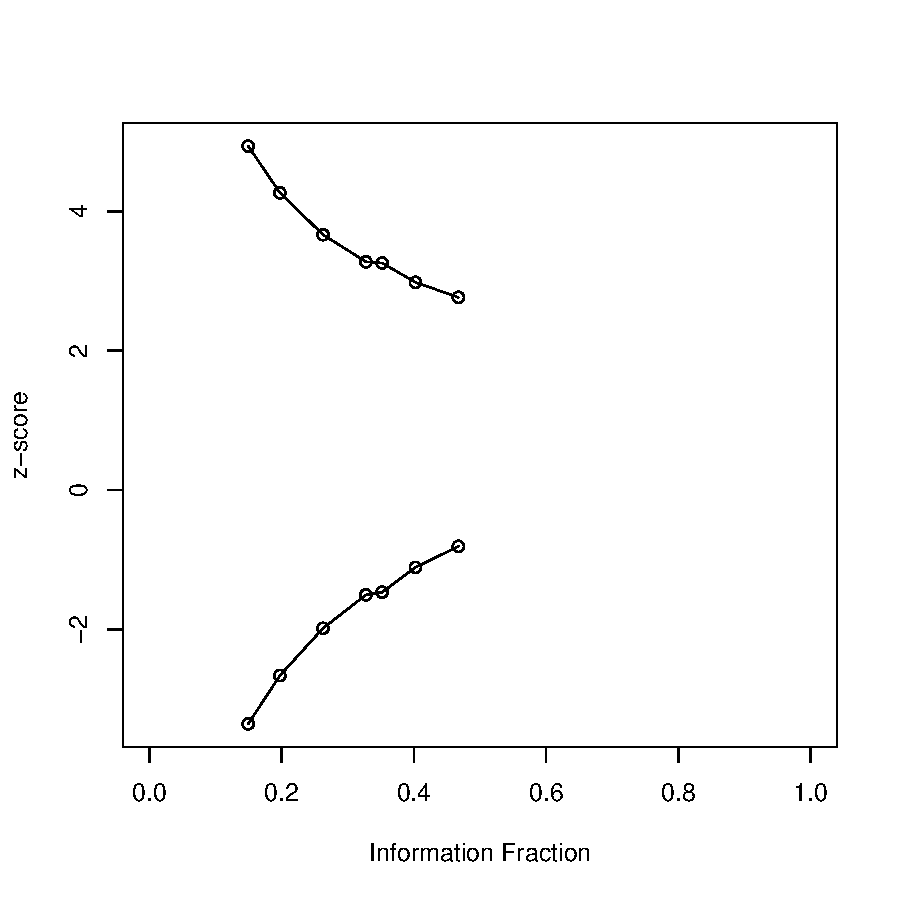
\includegraphics{GrpSeqBnds-vignette-1-incl-ex3-plot}
  \end{center}
  \caption{One-sided efficacy and futility boundaries constructed as in example 3, using the two
    information scales feature.  The main information scale in which the sequence of statistics is
    normalized to the scale of brownian paths, is the variance fraction, normalized to unity at
    the 7th analysis. The secondary scale upon which error probability is spent is the event ratio.}
  \label{fig:ex3}
  \end{figure}
  
  \item[4.]{{\bf Explore different boundary construction methods}\\
    Another boundary construction method is the one based upon the stochastic curtailment
    procedure. This results in boundaries which are typically more conservative at the
    begining but less so at the end as compared with the Lan-Demets boundaries based upon the
    O'Brien-Fleming spending function.
    
\begin{Schunk}
\begin{Sinput}
> example.4 <- example.3
> example.4$call$EfficacyBoundary <- as.call(expression(SC, 
+     alpha = 0.05, crit = 0.9))
> example.4 <- update(example.4)
> SimGSB(example.4)
\end{Sinput}
\begin{Soutput}
       eI.est       eI.act eII.est      eII.act
0.1494  0e+00 0.000000e+00 0.00003 2.090403e-05
0.1973  0e+00 1.607009e-10 0.00020 2.129657e-04
0.2625  0e+00 4.210657e-08 0.00137 1.325597e-03
0.3274  0e+00 1.263738e-06 0.00385 4.046323e-03
0.3519  0e+00 4.080870e-06 0.00534 5.558965e-03
0.4023  1e-05 1.888013e-05 0.00902 9.506958e-03
0.4673  5e-05 9.118187e-05 0.01590 1.612043e-02
\end{Soutput}
\end{Schunk}

\begin{Schunk}
\begin{Sinput}
> plot(example.4)
\end{Sinput}
\end{Schunk}

  \begin{figure}
  \begin{center}
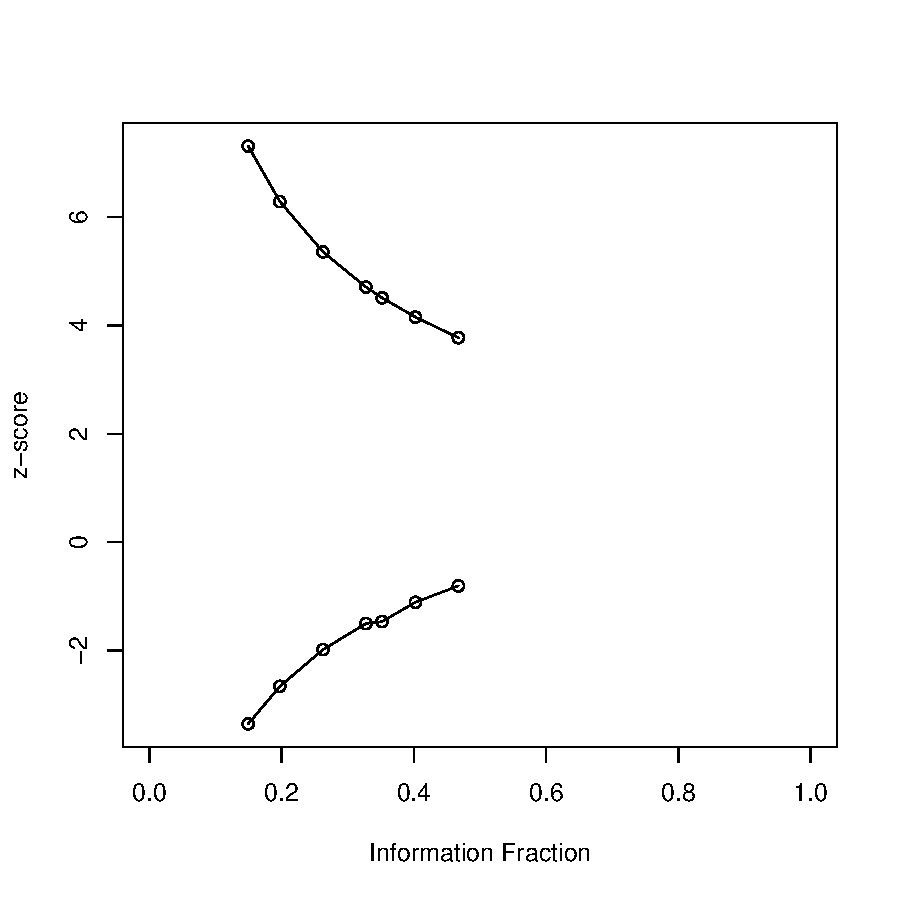
\includegraphics{GrpSeqBnds-vignette-1-incl-ex4-plot}
  \end{center}
  \caption{One-sided efficacy and futility boundaries constructed as in example 4, but this time 
    with efficacy boundary constructed according to the stochastic curtailment procedure.}
  \label{fig:ex4}
  \end{figure}
  
  Of course there are other options not covered in these examples but this should get you
    started.
  }
  \end{itemize}
\end{document}
